	\documentclass[a4paper,titlepage]{article}
	\usepackage[utf8]{inputenc}
	\usepackage[export]{adjustbox}
	\usepackage[french]{babel}
	\usepackage{hyperref}
	\usepackage{graphicx}
	\usepackage{fourier}
	\usepackage{color}   %May be necessary if you want to color links
	\usepackage{hyperref}
	\definecolor{GreyBlack}{RGB}{92, 89, 92}
	\hypersetup{
    		colorlinks=true, %set true if you want colored links
    		citecolor=black,
    		citecolor=black,
    		filecolor=black,
   			linkcolor=GreyBlack,
    		urlcolor=magenta
    }
	\usepackage[margin=1.3in]{geometry}
	\author{Baptiste Vergote & Martin Schreinemachers}
	\begin{document}
	% Page de titre
	\titlepage{
		16 Décembre 2014 \\[2cm]
		\begin{center}\sf\Huge
		{\bfseries \underline{Document 3 :}} \\[2mm]
		{\bfseries Langage avancé de programmation} \\[1cm]
		\begin{figure}[!h]
		\centering
			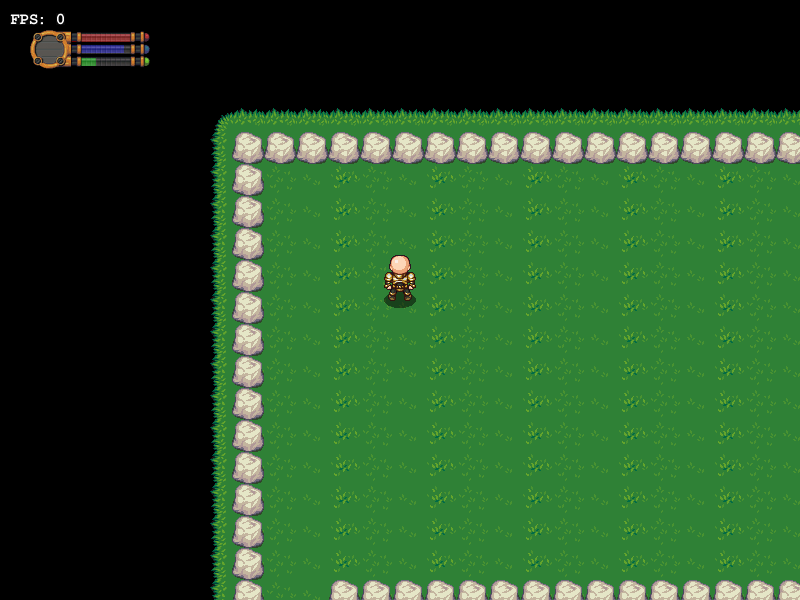
\includegraphics[scale=0.55]{carteJeu.png}
		\end{figure}
		\begin{center}
		{\huge RPG - The Epic School Adventure}
		
		\end{center}
		
		\end{center}
		\ \\[3.4cm]
		\textbf{Baptiste Vergote \& Martin Schreinemachers 2TL2} \\
		EPHEC LLN -- 2014-2015
	}
	\clearpage
	\tableofcontents
	\clearpage
	\section*{TODO}
	\begin{enumerate}
		\item Un document word comprenant : 
		\begin{enumerate}
			\item Une page de garde (noms, prénoms, class, titre du projet, un screenshot du projet, année académique).
			\item Une introduction où vous présentez votre projet.
			\item Le diagramme UML des classes OO que vous avez (ou un extrait intéressant).
			\item Un texte expliquant tout ce qui est nécessaire pour que votre projet fonctionne (modification du path, driver à installer et dans ce cas les fournir, …).
			\item Quelques screenshots de votre projet (idéalement pour illustrer des passages de votre travail – donc vous ne faites pas un titre screenshot mais vous en mettez là où c’est utile).
			\item Le code source (ou un extrait représentatif) documenté du package principal de l’application (+fichier package-info.java).
			\item La documentation du package principal (fichiers html générés par la javadoc).
			\item Une description de votre stratégie de validation.
			\item Une conclusion : que vous a apporté ce projet, quelles ont été les difficultés rencontrées, comment peut-on l’améliorer.
		\end{enumerate}
		\item Tous vos codes sources et tests unitaires (le projet eclipse).
		\item Le fichier JAR de votre application.
	\end{enumerate}
	\clearpage
	\section{Introduction}
	
	C’est dans une petite bourgade au plein centre du monde que j’attire votre attention... Tout a commencé dans les environs de Louvain-La-Neuve, en amont d’un lac, vide depuis un bon moment.\\

	Une journée bien trop remplie...Trois heures de suite à écouter un seul et même orateur parler de concepts et de notions cabalistiques. Un challenge que seuls peu, arrivent à endurer sans piquer du nez ! C’est dans cette ambiance somnolente, cet environnement âpre que débute l’aventure héroïque de nos deux programmeurs ! Dans cette pièce sombre et petite, où planent pêle-mêle, des effluves de transpirations, de cigarettes et de parfums, ils s’imaginent un monde idéal, où leurs héros seraient des rois devant leurs misérables vies de programmeur… Ils braveraient les démons et survivraient à ce monde hostile!\\

	C’est donc tout naturellement que le projet pris la forme d’un Jeu de Rôle. Tâche complexe, ardue du fait des nombreux facteurs, éléments à prendre en compte. C’est dans cette épreuve qu’ils se sont lancés.\\

	L’expédition de notre héros sera-t-elle un succès ? Serez vous capable de l’aider dans cette tache complexe? Parviendrez vous à l’amener au bout de son chemin? Serez vous assez fort pour les aider?\\
	
Réussirez-vous à arrêter toutes les menaces auxquels vous serez confrontés?
Si oui, suivez nous, arpentez vous dans ces contrées dangereuses et devenez protecteurs des faibles et des opprimés!

	
	\clearpage
	\section{Diagramme UML}
	Le diagramme complet est disponible en format PDF avec le nom UMLProjet (dans la partie rapport).
	\subsection{Package \og be.ephec.tesa.Personnage \fg{}  }	
	
	Dans ce package est compris tout ce qui constitue et gère les personnages :
	\begin{itemize}
		\item Dans \og Caract \fg{} le personnage se voit assigner 3 caractéristiques, à savoir la force, l'intelligence et l'endurance. Cette classe s'occupe de toute la gestion de ces caractéristiques.
		\item L' \og Équipement \fg{} est actuellement vide, il s'agit d'une classe ayant été créée en vue d'une implémentation future.
		\item L' \og Expérience \fg{} gère comme son nom l'indique, l'expérience du personnage et ses niveaux.
		\item Les \og MonstresCommuns \fg{} et \og MonstresElites \fg{} sont les classes qui permettent de manier les ennemis du personnage.
	\end{itemize}
	\begin{figure}[h!]
		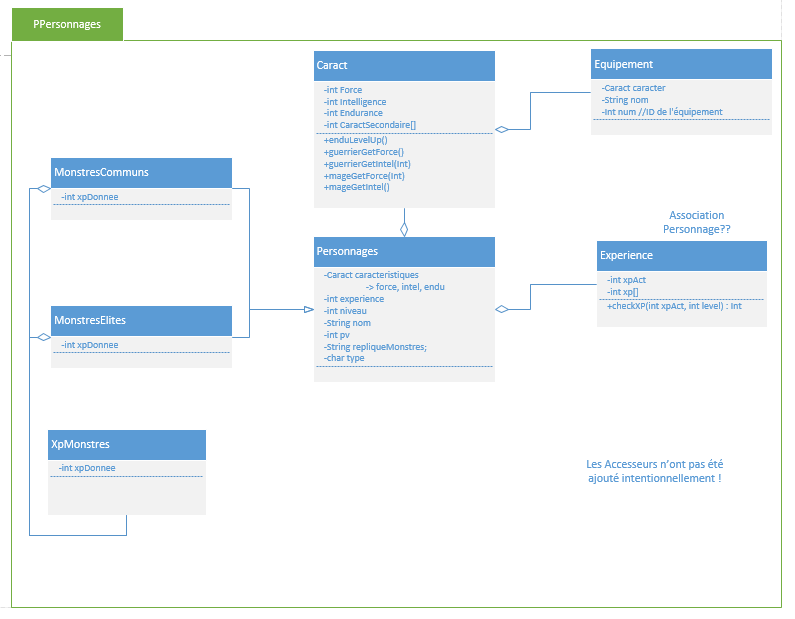
\includegraphics[scale=0.80]{PPersonnage.png}
	\end{figure}
	
	\newpage
	\subsection{Package \og be.ephec.tesa.main \fg{} \& \og be.ephec.tesa.jdbc \fg{} }
	Ce package contient plusieurs classes :
	\begin{itemize}

		\item \og Jeu \fg{} contient tous les états et permet de lancer le jeu.
		\item \og initPartie \fg{} qui initialise les monstres et les joueurs.
		\item \og Combat \fg{} s'occupe de la gestion de tous les combats.
		\item \og Player \fg{} détermine l'animation et les mouvements du joueur sur la carte d'un point de vue graphique.
		\item \og PlayerController \fg{} permet de contrôler les mouvements du joueur d'un point de vue logique.
		\item \og TriggerController \fg{} qui va gérer les collisions et les changements de carte.
		\item et finalement \og CONSTANTES \fg{} qui contient toutes les constantes du programme.
	\end{itemize}	
	\ 
		
	La gestion de la base de données se fait dans le package \og be.ephec.jdbc \fg{}, c'est la que sont effectuées et traitées les Query.	
	\ \\
	\begin{figure}[h!]
		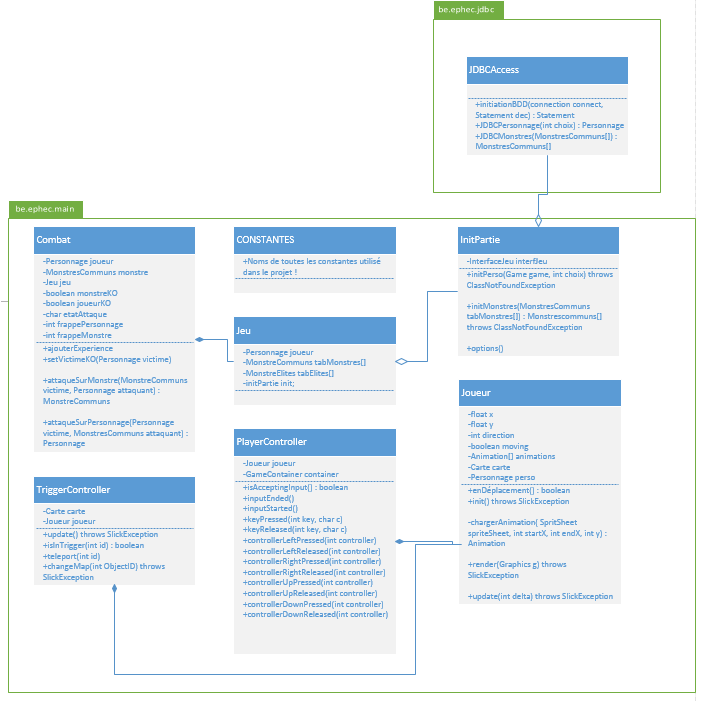
\includegraphics[scale=0.85]{Pjdbc&Pmain.png}
	\end{figure}

	\newpage
	\subsection{Package \og be.ephec.tesa.gui \fg{} }
	Les classes de ce package sont :
	\begin{itemize}
		\item \og Camera \fg{} qui permet que la vision suive le joueur sur la carte.
		\item \og Carte \fg{} définit la carte sur lequel le personnage se meut. 
		\item \og HUD \fg{}  affiche les barres de vie, de mana et d'expérience du personnage.
		\item \og InterfaceCarte \fg{} affiche la carte et gère les déplacements des personnages sur la carte.
		\item \og InterfaceIntro \fg{} gère tout ce qui est relatif à l'affichage de la page d'introduction.
		\item \og InterfaceCreationPersonnage \fg{} gère tout ce qui est relatif à la création du personnage.
		\item \og interfaceCombat \fg{} gère tout ce qui est relatif à l'affichage d'un combat.
		\item \og InterfaceJeu \fg{} gère tous les états du jeu (l'introduction du jeu, la création du personnage, le déplacement dans le monde et le combat et le GameOver)
	\end{itemize}
	\begin{figure}[h!]
		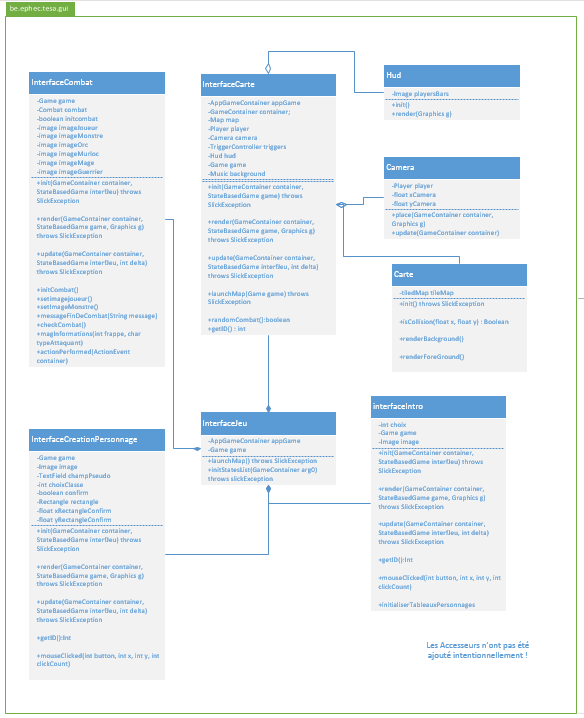
\includegraphics[scale=0.92]{Pgui.png}
	\end{figure}
	\clearpage
	
	\section{Necessité pour la fonctionnalité}
	Un texte expliquant tout ce qui est nécessaire pour que votre projet fonctionne (modification du path, driver à installer et dans ce cas les fournir, …).
	\clearpage
	
	\section{Notre jeu étapes par étapes}
	En double cliquant sur le fichier JAR, le jeu se lance en plein écran, vous laissant apercevoir un magnifique écran de démarrage :
	\begin{figure}[h!]
		\includegraphics[scale=0.30]{EcranDebut.jpg}
	\end{figure}
	
	Sur cette image, trois boutons sont présents : 
	\begin{enumerate}
		\item Le bouton de création d'une Nouvelle Partie.
		\item La bouton permettant de Continuer la partie en cours.
		\item Un bouton pour changer les options.
	\end{enumerate}
	
	En cliquant sur "Nouvelle Partie", un écran de sélection de personnage apparait :
	\begin{figure}[h!]
		\includegraphics[scale=0.30]{EcranCreationPersonnage.jpg}
	\end{figure}
	
	Vous cliquez sur le personnage que vous souhaitez jouer, lui entrez un Pseudo et le jeu commence :
	\begin{figure}[h!]
		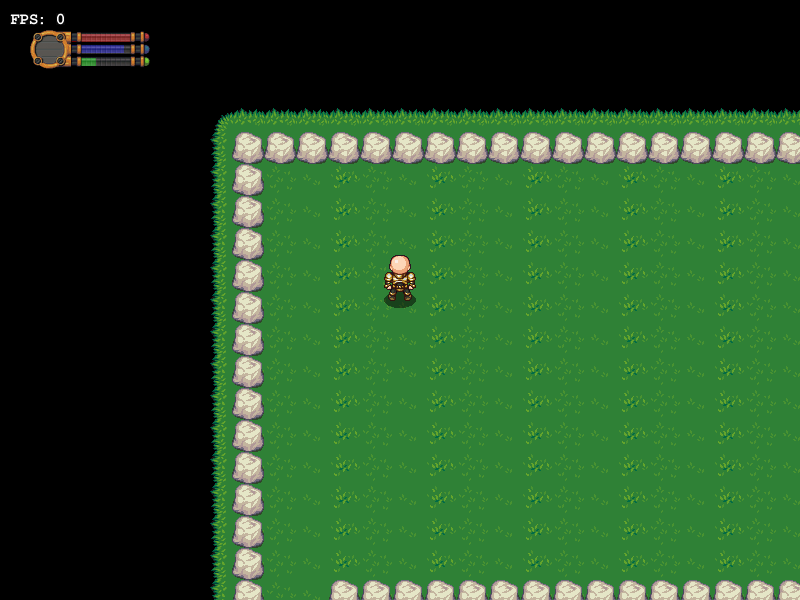
\includegraphics[scale=0.65]{carteJeu.png}
	\end{figure}
	
	Comme vous pouvez le constater, le guerrier apparait dans le coin supérieur gauche de la carte, celle-ci délimitée par les petits cailloux que vous ne pourriez, bien entendu, pas traverser ;) !\\
	
	En se baladant dans la prairie, celui ci va se heurter à des rencontres inattendues ou notre champion va devoir vendre chèrement sa peau !\\
	
	Nous ne dévoilerons pas la suite, à vous de la découvrir !\\
	
	Bonne chance dans cet univers rempli de monstres sanguinaires !
	\clearpage
	
	\section{Documentation du package}
	La documentation du package principal (fichiers html générés par la javadoc).
	\clearpage
	
	\section{Description de la stratégie de validation}
	Tout d’abord, nous avons commencé par parler ensemble de ce que nous voulions comme éléments dans notre jeu : quel personnage, quel spécificité lui donner, quels adversaires, quels possibilités d’actions...Nous avons rassemblé le tout sur une feuille en un semblant de diagramme UML.\\

Après avoir laissé mûrir le projet dans notre réflexion, nous avons fait un schéma UML complet et nous avons commencé à réfléchir à la structure de la base de données devant accueillir les données relatives à notre jeu. Nous avons alors attaqué l’implémentation du jeu.	
\clearpage
	
	\section{Difficultés rencontrées}
	La première difficulté pour nous était d’appréhender le problème de conception de notre jeu. Quels éléments intégrer (monstres de différents types ? Leur permettre de sortir des répliques ? Implémenter un système d’équipements ?), comment les intégrer, comment séparer tout ces éléments logique en classes…\\
	
Rapidement suivi par nos débuts avec les interfaces graphiques. D’abord, nous sommes partis sur une interface plus simple utilisant les libraires swing, sur le conseil d’un camarade, nous nous sommes redirigés vers les librairies Slick2d qui facilitent grandement l’implémentation de jeu en 2D.\\

Pour Slick2d, la difficulté résidait d’abord dans le fait qu’on utilisait des classes écrites par d’autres et dont on ne voit pas toujours le code...\\ L’habitude venant avec la pratique, ce problème s’est rapidement résolu pour la plupart des cas. Vient ensuite une bêtise qui nous à fait perdre beaucoup de temps : Slick2d \og réinvente \fg{} Java. Pour indiquer un chemin vers une image, un fichier de musique, il faut commencer par le nom du dossier $/$ du fichier lui-même alors qu'habituellement, on indique le début d’un chemin par un \og $/$ \fg{}. \\

Autre perte de temps, les coordonnées des objets sont calculées à partir du coin inférieur gauche de l’écran, et non à partir du coin supérieur gauche...\\

Les classes que nous avons utilisés dans Slick2d nous ont permis de créer un jeu basé sur des états, ceux-ci déterminant chacun un écran et une étape de jeu.
	\section{Conclusion}
	\textit{Une conclusion : que vous a apporté ce projet, quelles ont été les difficultés rencontrées, comment peut-on l’améliorer.}\\
	\\
	\\ \url{http://www.lirmm.fr/~coletta/TER/Rapport-TER.pdf} \\
	 Exemple de conclusion (pg 27 / 29)
	 \\
	 \\
	 \textbf{J'AJOUTE JUSTE DES IDEES : MODIFIABLE AS FUCK}\\
	\\
	Nous avons réalisé, dans le cadre du cours de  un jeu de type RPG ayant comme principal sujet l'EPHEC et ses étudiants. Les monstres communs seront des étudiants fictifs des différentes sections de l'EPHEC (à savoir : Comptabilité, Commercial, Business, Droit, Marketing). Les monstres élites seront des professeurs fictifs de la section TI de Louvain-La-Neuve.
	Martin adorait l'idée d'un RPG, étant tous les deux des joueurs de RPG, nous nous sommes lancés très vite dans l'idée.
	\\
	\\
	Malgré quelques difficultés à cerner le problème initial, nous avons persevérer pour parvenir au jeu actuel.
	\\
	\\
	Après plus de 2 ans à faire des "petits programmes" sans grand intéret, enfin nous apprenons et réalisons un programme entier! Il s'agit d'un grand progrès qui nous aura maintenu motivé jusqu'au bout !
	\\
	\\
	Si notre programme rencontre du succès, nous pourrions imaginer le développer plus en profondeur en ajoutant par exemple, l'utilisation d'équipement, laché par les monstres, qui boosterait les caractéristiques du héros
	\\
	\\
	Ce projet nous a permis d'appliquer toutes les connaissances apprises lors de nos deux années à l'EPHEC...
	
	\clearpage
	\section*{Sources }
\danger Nous ne nous sommes pas préoccupés, dans le cadre de ce projet des éventuels droits d'auteurs.\\

Il est aussi important de préciser que les images ont été redimmensionné et parfois coupé pour les besoins de ce projet.	
	
\subsubsection*{Bibliographie :}

\begin{itemize}
	\item Les bibliothèques de l'université de Louvain-La-Neuve. (2013) \textit{Rédiger une bibliographie au format APA.} Lien du PDF sur : \url{http://www.uclouvain.be/cps/ucl/doc/bpsp/documents/Bibliographie\_APA\_F\_13doi.pdf},  consultée le 13 décembre 2014.
	\item Pharmacritique. (2009). \textit{Le rapport de l'IGAS donne une idée des conflits d'intérêts financiers des médecins travaillant pour l'industrie et des intérêts autres qui biaisent la recherche médicale.} En ligne sur \url{http://pharmacritique.20minutes-blogs.fr/archive/2009/02/07/le-rapport-de-l-igas-nous-donne-une-idee-des-conflits-d-inte.html}, consultée le 10 décembre 2014.
	\item La pub de tropicalboy. (2006). \textit{Royal Canin}. En ligne sur \url{http://mapubamoi.canalblog.com/archives/2006/04/13/1694142.html}, consultée le 10 décembre 2014.
	\item Le devoir, libre de penser. (2007). \textit{Les caricatures de Garnotte}. En ligne sur \url{http://www.ledevoir.com/galeries-photos/les-caricatures-de-garnotte/71304}, consultée le 10 décembre 2014.
	\item Les experts Denjean associés. (2014). \textit{Quiz : Quel professionnel comptable êtes-vous?} En ligne sur \url{http://www.les-experts-denjean-associes.com/test-quel-genre-dexpert-comptable-etes-vous/}, consultée le 10 décembre 2014.
	\item Funny Art Pictures. (2008). \textit{Ultimate Attraction.} En ligne sur \url{http://www.funnyartpictures.com/pics-funny-stuff/?images/midsize/signs-ads/ultimate-attraction.jpg}, consultée le 10 décembre 2014.
	\item GoPixPic. (Date inconnue). \textit{Games Returns In the Guild Wars 2...} En ligne sur \url{http://www.gopixpic.com/640/-games-returns-in-the-guild-wars-2-warrior-classes/http:||guides*gamepressure*com|guildwars2|gfx|word|978182984*jpg/}, consultée le 1 décembre 2014.
	\item Guild Wars 2 - Profession - Élémentaliste. (Date inconnue entre 2010 et 2014). \textit{Fond d'écran - Élémentaliste.} En ligne sur \url{https://www.guildwars2.com/fr/the-game/professions/elementalist/}
	\item Color picker with high precision and contrast test. (Date inconnue) \textit{Color picker.} En ligne sur \url{http://colorizer.org/}, consultée le 1 décembre 2014.
	\item OpenClassrooms. (Date inconnue). \textit{Apprenez à programmer en Java - Positionner des boutons.} En ligne sur \url{http://openclassrooms.com/courses/apprenez-a-programmer-en-java/positionner-des-
boutons}
	\item Wikipédia. (Dernière modification le 10 décambre 2014). \textit{Noms de couleur du Web.} En ligne sur \url{http://fr.wikipedia.org/wiki/Couleurs_du_Web}.
	\item Apprendre Java - Cours et exercices. (2011). \textit{Les interfaces graphiques en Java.} En ligne sur \url{http://www.infres.enst.fr/~hudry/coursJava/interSwing/index.html}
	\item Open Game Art. (Date inconnue) \textit{Morning Sunrise Background.} En ligne sur \url{http://opengameart.org/content/morning-sunrise-background}
	\item Shionn::blog() - Be a geek. (Date inconnue). \textit{Tutoriels slick 2D.} En ligne sur \url{http://www.shionn.org/tutoriels-slick-2d}
\end{itemize}
	
	\clearpage	
	\end{document}